\begin{enumerate}[\Large\bfseries 1.]

%--------------------1.
\item \textbf{\large LÍMITES}\\\\

    \begin{enumerate}[\bfseries a)]

	%----------a.
	\item \textbf{\large Michael Spivak, Calculus, capítulo 5}\\\\
	Hallar los siguientes limites (Estos limites se obtienen todos, después de algunos cálculos, de las distintas partes del teorema 2; téngase cuidado en averiguar cuáles son las partes que se aplican, pero sin preocuparse de escribirlas.)\\\\
	$$\lim\limits_{x \to 1}\dfrac{x^2-1}{x+1} = \dfrac{1^2 - 1}{1 + 1} = \dfrac{0}{2} = 0$$\\\\

	%----------b)
	\item \textbf{Código fuente.}\\ 
	    
	    \lstinputlisting[language=Python]{python/tareas_mat/week5/limit1.py}
	    \vspace{.5cm}
	
	%----------c)
	\item \textbf{Prueba de la ejecución del programa}.\\
	    \begin{center}
		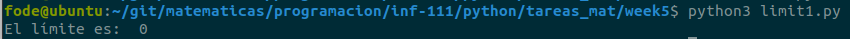
\includegraphics[scale=.55]{imagenes/tareas_mat/week5/limit1.png}
	    \end{center}

    \end{enumerate}

\newpage

%--------------------2.
\item \textbf{\large LÍMITES}\\\\

    \begin{enumerate}[\bfseries a)]

	%----------a.
	\item \textbf{\large Michael Spivak, Calculus, capítulo 5}\\\\
	Hallar los siguientes limites (Estos limites se obtienen todos, después de algunos cálculos, de las distintas partes del teorema 2; téngase cuidado en averiguar cuáles son las partes que se aplican, pero sin preocuparse de escribirlas.)\\\\
	$$\lim\limits_{x \to 2} \dfrac{x^3 - 8}{x - 2} = \dfrac{(x-2)(x^2+2x+4)}{x-2} = 2^2+4+4 = 12$$\\\\

	%----------b)
	\item \textbf{Código fuente.}\\ 
	    
	    \lstinputlisting[language=Python]{python/tareas_mat/week5/limit2.py}
	    \vspace{.5cm}
	
	%----------c)
	\item \textbf{Prueba de la ejecución del programa}.\\
	    \begin{center}
		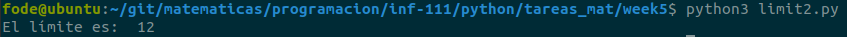
\includegraphics[scale=.5]{imagenes/tareas_mat/week5/limit2.png}
	    \end{center}

    \end{enumerate}

\newpage

%--------------------3.
\item \textbf{\large LÍMITES}\\\\

    \begin{enumerate}[\bfseries a)]

	%----------a.
	\item \textbf{\large Michael Spivak, Calculus, capítulo 5}\\\\
	Hallar los siguientes limites (Estos limites se obtienen todos, después de algunos cálculos, de las distintas partes del teorema 2; téngase cuidado en averiguar cuáles son las partes que se aplican, pero sin preocuparse de escribirlas.)\\\\
	$$\lim\limits_{x \to 3} \dfrac{x^3-8}{x-2} = \dfrac{3^3-8}{3-2} =19$$\\\\

	%----------b)
	\item \textbf{Código fuente.}\\ 
	    
	    \lstinputlisting[language=Python]{python/tareas_mat/week5/limit3.py}
	    \vspace{.5cm}
	
	%----------c)
	\item \textbf{Prueba de la ejecución del programa}.\\
	    \begin{center}
		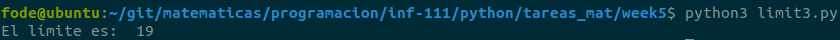
\includegraphics[scale=.5]{imagenes/tareas_mat/week5/limit3.png}
	    \end{center}

    \end{enumerate}

\newpage

%--------------------4.
\item \textbf{\large LÍMITES}\\\\

    \begin{enumerate}[\bfseries a)]

	%----------a.
	\item \textbf{\large Michael Spivak, Calculus, capítulo 5}\\\\
	    Hallar el límite de: \\\\
	    $\lim\limits_{x \to 1} \dfrac{1-\sqrt{x}}{1-x} =\lim\limits_{x \to 1} \dfrac{1-\sqrt{x}}{1-x}\cdot \dfrac{1+\sqrt{x}}{1+\sqrt{x}} =\lim\limits_{x \to 1} \dfrac{1^2 - (\sqrt{x})^2}{(1-x)(1+\sqrt{x})} =\lim\limits_{x \to 1} \dfrac{1}{1+\sqrt{x}} = \dfrac{1}{2}$\\\\
    
	%----------b)
	\item \textbf{Código fuente.}\\ 
	    
	    \lstinputlisting[language=Python]{python/tareas_mat/week5/limit4.py}
	    \vspace{.5cm}
	
	%----------c)
	\item \textbf{Prueba de la ejecución del programa}.\\
	    \begin{center}
		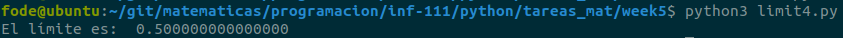
\includegraphics[scale=.5]{imagenes/tareas_mat/week5/limit4.png}
	    \end{center}

    \end{enumerate}

\newpage

%--------------------5.
\item \textbf{\large LÍMITES}\\\\

    \begin{enumerate}[\bfseries a)]

	%----------a.
	\item \textbf{\large Michael Spivak, Calculus, capítulo 5}\\\\
	    Hallar el límite de:\\\\
	    $\lim\limits_{x \to 0} \dfrac{1-\sqrt{1-x^2}}{x} =\lim\limits_{x \to 0} \dfrac{1-\sqrt{1-x^2}}{x} \cdot \dfrac{1+\sqrt{1-x^2}}{1+\sqrt{1-x^2}} =\lim\limits_{x \to 0} \dfrac{x}{1+\sqrt{1-x^2}} = 0$\\\\

	%----------b)
	\item \textbf{Código fuente.}\\ 
	    
	    \lstinputlisting[language=Python]{python/tareas_mat/week5/limit5.py}
	    \vspace{.5cm}
	
	%----------c)
	\item \textbf{Prueba de la ejecución del programa}.\\
	    \begin{center}
		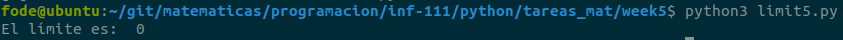
\includegraphics[scale=.5]{imagenes/tareas_mat/week5/limit5.png}
	    \end{center}

    \end{enumerate}

\newpage

%--------------------6.
\item \textbf{\large LÍMITES}\\\\

    \begin{enumerate}[\bfseries a)]

	%----------a.
	\item \textbf{\large Michael Spivak, Calculus, capítulo 5}\\\\
	    Hallar el límite de: \\\\
	    $\lim\limits_{x \to 0} \dfrac{1-\sqrt{1-x^2}}{x^2} = \lim\limits_{x \to 0} \dfrac{1-\sqrt{1-x^2}}{x^2}\cdot \dfrac{1+\sqrt{1-x^2}}{1+\sqrt{1-x^2}} = \lim\limits_{x \to 0} \dfrac{1}{1+\sqrt{1+x^2}} = \dfrac{1}{2}$\\\\

	%----------b)
	\item \textbf{Código fuente.}\\ 
	    
	    \lstinputlisting[language=Python]{python/tareas_mat/week5/limit6.py}
	    \vspace{.5cm}
	
	%----------c)
	\item \textbf{Prueba de la ejecución del programa}.\\
	    \begin{center}
		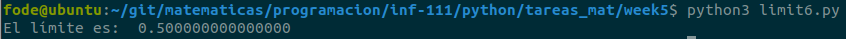
\includegraphics[scale=.5]{imagenes/tareas_mat/week5/limit6.png}
	    \end{center}

    \end{enumerate}

\newpage
\end{enumerate}
